% !Mode:: "TeX:UTF-8"
\documentclass{../../common/tufte-latex/tufte-handout}

\title{Git en Pratique, partie II-c: R\'e-\'ecrire l'Historique}
\author{S\'ebastien Dawans}

\date{4 Ao\^ut 2015} % without \date command, current date is supplied

%\geometry{showframe} % display margins for debugging page layout
\usepackage[utf8]{inputenc}
\usepackage{graphicx} % allow embedded images
  \setkeys{Gin}{width=\linewidth,totalheight=\textheight,keepaspectratio}
  \graphicspath{{graphics/}} % set of paths to search for images
\usepackage{amsmath}  % extended mathematics
\usepackage{booktabs} % book-quality tables
\usepackage{units}    % non-stacked fractions and better unit spacing
\usepackage{multicol} % multiple column layout facilities
\usepackage{lipsum}   % filler text
\usepackage{fancyvrb} % extended verbatim environments
  \fvset{fontsize=\normalsize}% default font size for fancy-verbatim environments
\usepackage{listings}
\lstset{showstringspaces=false}
\usepackage[usenames]{xcolor}
\usepackage{hyperref}

\lstdefinestyle{BashInputStyle}{
  language=bash,
  basicstyle=\footnotesize\ttfamily,
  %numbers=left,
  %numberstyle=\tiny,
  %numbersep=3pt,
  frame=tb,
  columns=fullflexible,
  backgroundcolor=\color{yellow!20},
  linewidth=0.95\linewidth,
  xleftmargin=0.05\linewidth,
  moredelim=**[is][\color{red}]{§}{§},
  moredelim=**[is][\color{OliveGreen}]{`}{`}
}

% Standardize command font styles and environments
\newcommand{\doccmd}[1]{\texttt{\textbackslash#1}}% command name -- adds backslash automatically
\newcommand{\docopt}[1]{\ensuremath{\langle}\textrm{\textit{#1}}\ensuremath{\rangle}}% optional command argument
\newcommand{\docarg}[1]{\textrm{\textit{#1}}}% (required) command argument
\newcommand{\docenv}[1]{\textsf{#1}}% environment name
\newcommand{\docpkg}[1]{\texttt{#1}}% package name
\newcommand{\doccls}[1]{\texttt{#1}}% document class name
\newcommand{\docclsopt}[1]{\texttt{#1}}% document class option name
\newenvironment{docspec}{\begin{quote}\noindent}{\end{quote}}% command specification environment

\begin{document}

\maketitle% this prints the handout title, author, and date

\begin{abstract}
\noindent
Ce document est un complément à la \texttt{Partie II: Op\'erations en solo}.
Il montre quelques possibilités offertes par les fonctionalités de ré-écriture d'historique de Git.
\end{abstract}

\section{Un homme averti en vaut deux}

Avant de découvrir les merveilles de l'édition d'historique de Git, notons que ce privilège doit être utilisé avec sagesse.

Changer l'historique d'une branche \textbf{déjà partagées avec d'autres développeurs} n'est pas une bonne pratique, parce que ces personnes devront exécuter \texttt{git reset -{}-hard} (ou autres commandes selon les cas) pour réintégrer vos changements dans leur historique.

\begin{marginfigure}%
  \centering
  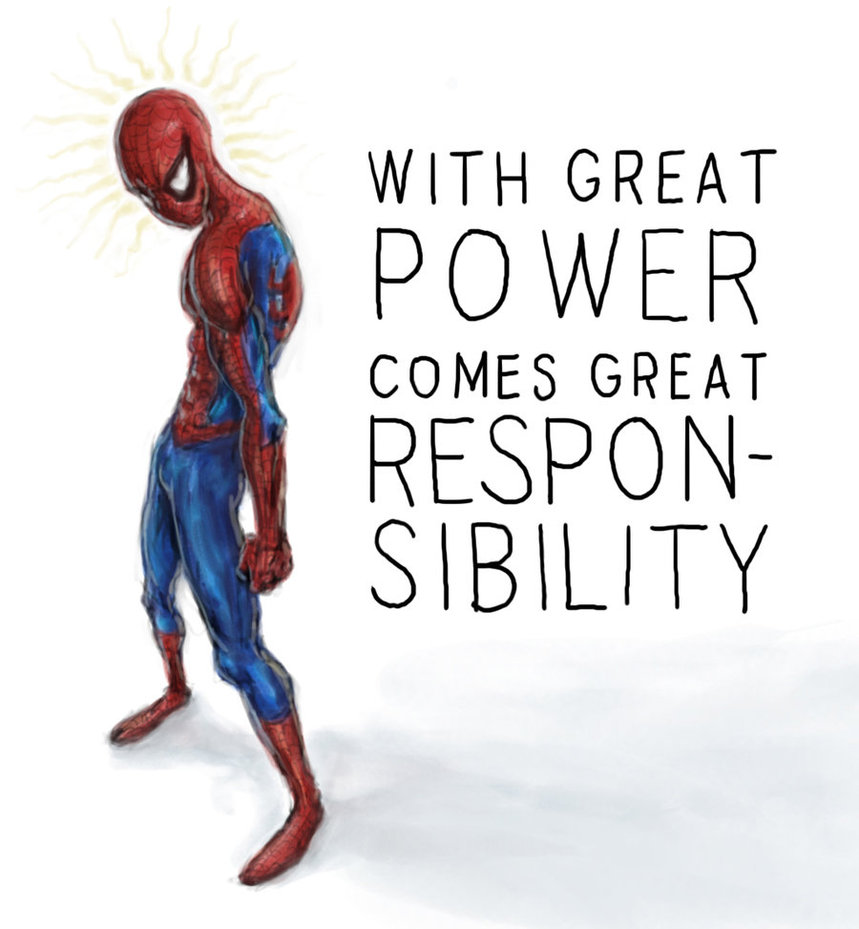
\includegraphics[width=\linewidth]{spiderman.jpg}
  \label{fig:spiderman}
\end{marginfigure}

L'édition d'historique est un moyen pratique de faire le ménage avant de contribuer du code, mais ne doit pas être appliqué a posteriori sur une branch importante (master, develop). \marginnote{en lisant entre les lignes: il est toléré de forcer une ré-écriture sur vos branches personelles, mais mieux vaut ne pas prendre l'habitude.} Git prévoit un garde-fou au cas ou vous outre-passiez cette règle de bonne pratique, volontairement ou non: il faut obligatoirement inclure l'option \texttt{-{}-force} sur la commande \texttt{push} lorsqu'un changement d'historique est appliqué sur une branche déjà précédemment pushée.

En cas de doute sur cette règle, retenez simplement \textbf{qu'il faut éviter de modifier l'historique d'une section de branche déjà partagée sur un repo distant}.

\section{Ré-écrire l'Historique}
Git offre la possibilité de ré-écrire l'historique, mais en quoi cela consiste-il? Quelles sont les opérations qui résultant en un changement d'historique? C'est ce que nous nous apprêtons à voir.

Changer l'historique peut être: \textbf{l'édition d'un message} de commit, la \textbf{combinaison} de commits, la \textbf{séparation} d'un gros commit en plusieurs commits distincts, la \textbf{suppression} d'un commit, la modification de meta-données du commit (\textbf{date, auteur}), la \textbf{modification du contenu} d'un commit (ajouter/supprimer une ligne de code), etc...

\subsection{Modifier le denier commit}
La forme la plus simple de modificationd d'historique est la modification du dernier commit.

\begin{lstlisting}[style=BashInputStyle]
  $ git commit --amend
\end{lstlisting}

Cette commande ouvre un éditeur de texte vous permettant d'éditer le message du dernier commit.
Elle prend également tout ce que a été déplacé dans l'index depuis le dernier commit (via \texttt{git add}) et le combine avec le commit précédent plutôt que d'en créer un nouveau.
Nous voyons que cela peut avoir deux rôles: \textbf{l'édition du dernier message de commit} et \textbf{la modification du contenu du dernier commit}.

Modifions le dernier message de commit de la branche master du repo lesson1:

\begin{lstlisting}[style=BashInputStyle]
  $ git clone git@gitlab.server.com:login/lesson1
  $ cd lesson1
  $ git checkout master # facultatif
  $ git log --oneline
  $ gitk --all
  $ git commit --amend -m "New message"
  $ git log --oneline
  $ gitk --all
\end{lstlisting}

\begin{figure*}%
  \centering
  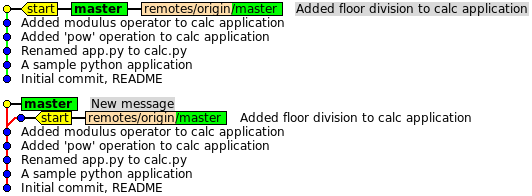
\includegraphics[width=0.85\linewidth]{gitcommit-amend.png}
  \label{fig:gitcommit-amend}
  \caption{Avant (haut) et après (bas) la modification du dernier message de commit}
\end{figure*}

La sortie de \texttt{gitk} aux deux étapes est ilustrée à la Figure \ref{fig:gitcommit-amend}.
Nous voyons que la modification du dernier message de commit entraîne une divergence entre notre branche \texttt{master} locale et la branche \texttt{master} du repository distant \texttt{origin}.
Le changement d'historique signifie que \textbf{vous ne pouvez plus push} sans l'option \texttt{--force}. \marginnote{Comme le HASH d'un commit englobe l'état du working tree ainsi que les méta-données du commit (auteur, date, message...), changer l'une des ces information est considéré comme une modification d'historique.}
D'un autre point de vue: Git refusera de remplacer la branche \texttt{master} distante par votre nouvelle branche car le dernier commit de la branche master distante n'est pas dans l'historique direct de votre branche master locale.

\subsection{Des modifications plus importantes avec le rebase interactif}

Editer le dernier commit n'est qu'une petite fraction des possibilités offertes par Git. Une approche plus puissante et plus générale est la modification de l'historique via la commande \texttt{rebase}, en mode interactif.

Le fait de \textbf{rebase} votre HEAD sur un \texttt{tree-ish} particulier, demandera à Git de:

\begin{enumerate} 
 \item{remonter l'historique de votre propre HEAD et du tree-ish demandé jusqu'à obtenir un ancêtre commun}
 \item{lister les commits entre l'ancêtre commun et HEAD, et de les appliquer dans le même ordre par dessus le tree-ish spécifié}
 \item{après chaque commit, déplacer le pointeur de HEAD sur le nouveau commit avant d'appliquer le commit suivant.}
\end{enumerate}

C'est une commande très générale et utile dans plusieurs contextes différents.
Lors de la troisième étape, quand Git applique chaque commit sur le tree-ish de destination, il est possible de demander d'exécuter une opétation supplémentaire à chaque commit en invoquant le \textbf{rebase en mode interactif}.
C'est particulièrement utile pour ré-écrire l'historique d'une branche: il suffit de \texttt{rebase} la branche sur un HASH dans son historique directe.

Supposons que nous voulions altérer les messages de commit de HEAD\textasciitilde1 et HEAD\textasciitilde2, nous ferions:

\marginnote{HEAD\textasciitilde n est un raccourcis pour désigner le n+1ème dernier commit (i.e. n commits derrière le dernier commit)}
\begin{lstlisting}[style=BashInputStyle]
  $ git rebase -i HEAD~3
\end{lstlisting}

Cela revient à prendre HEAD et de la rebase sur un commit qui est 3 commits en arrière dans l'historique. Cela défera HEAD, HEAD\textasciitilde1 et HEAD\textasciitilde2, et préparera Git à les réappliquer dans l'ordre inverse sur le commit HEAD\textasciitilde3 (l'ordre sera HEAD\textasciitilde2, HEAD\textasciitilde1 et HEAD). \marginnote{sans l'option -i, cela revient à ne rien modifier}
Avec l'option -i, un éditeur de texte s'ouvrira pour vous demander de préciser l'opération à appliquer sur chaque commit:

\begin{lstlisting}[style=BashInputStyle]
  pick 21471dd Added 'pow' operation to calc application
  pick 511d31d Added modulus operator to calc application
  pick 87854e9 New message
\end{lstlisting}

Nous souhaitons modifier deux des commit - pour cela, nous remplaçons 'pick' par une nouvelle opération, 'edit' (ou 'e', tout simplement):

\begin{lstlisting}[style=BashInputStyle]
  edit 21471dd Added 'pow' operation to calc application
  edit 511d31d Added modulus operator to calc application
  pick 87854e9 New message
\end{lstlisting}

Une fois cet éditeur fermé, Git effectuera le rebase en appliquant les commits les uns après les autres sur le commit HEAD\textasciitilde3, en s'arrêtant pour exécuter l'opération demandée.
La première action est d'appliquer et éditer le commit 21471dd, donc Git s'arrêtera pour vous signaler qu'il est possible d'éditer le commit:

\begin{lstlisting}[style=BashInputStyle]
Stopped at 21471dd... Added 'pow' operation to calc application
You can amend the commit now, with

	git commit --amend

Once you are satisfied with your changes, run

	git rebase --continue
\end{lstlisting}

Suivons ces conseil: modifions le dernier message de commit, puis poursuivons le rebase:

\begin{lstlisting}[style=BashInputStyle]
git commit --amend -m "New commit message 1"
git rebase --continue
\end{lstlisting}

Cela nous vaudra un message de Git similaire au précédent, car il se sera arrêté au commit 511d31d.
Nous allons une nouvelle fois éditer le dernier commit et poursuivre le rebase:

\begin{lstlisting}[style=BashInputStyle]
git commit --amend -m "New commit message 2"
git rebase --continue
\end{lstlisting}

Git prendra automatiquement le dernier commit avant de clôturer l'opération de rebase, car nous avons demandé un simple 'pick'.
L'historique final après le premier \texttt{amend} suivi du \texttt{rebase} interactif est illustré à la Figure \ref{fig:gitrebase-amend}.

\begin{figure*}%
  \centering
  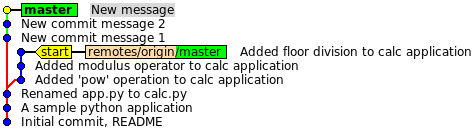
\includegraphics[width=0.75\linewidth]{gitrebase-amend.png}
  \label{fig:gitrebase-amend}
  \caption{Nouvel historique après avoir modifié les 3 derniers messages de commit}
\end{figure*}

\noindent Nous avons couvert le mécanisme générale de git rebase en mode interactif. Nous allons maintenant apercevoir quelques opérations plus avancées que permet le rebase interactif.
Premièrement, annulons nos dernières modifications en réinitialisant notre branche \texttt{master} locale à l'état de la branche \texttt{origin/master}:

\begin{lstlisting}[style=BashInputStyle]
  git reset --hard origin/master
\end{lstlisting}

\noindent \textbf{Combiner des commits}.
Plusieurs commits peuvent être aggrégés en un seul commit.

Pour cela, utilisons l'option \textbf{squash} dans l'éditeur du rebase interactif.
Combinons les commits HEAD\textasciitilde1 et HEAD\textasciitilde2

\begin{lstlisting}[style=BashInputStyle]
  $ git rebase -i HEAD~3
\end{lstlisting}

Cette fois, nous modifions l'éditeur de rebase de la manière suivante:

\marginnote{Le \textbf{squash} combine un commit avec le précédent, donc il faut préciser squash sur le commit du \textbf{bas}.}
\begin{lstlisting}[style=BashInputStyle]
  pick 21471dd Added 'pow' operation to calc application
  squash 511d31d Added modulus operator to calc application
  pick 87854e9 New message
\end{lstlisting}

Lors de rebase, Git appliquera 21471dd tel quel, puis l'ammendera en le combinant avec le contenu de 511d31d.
Un éditeur vous donnera la possibilité de choisir un message de commit pour ce nouveau commit combiné:

\marginnote{Git squash est plutôt bien fait: si vous faites un squash de plusieurs commits consécutifs, ils apparaîtront tous ici en une fois.}
\begin{lstlisting}[style=BashInputStyle]
# This is a combination of 2 commits.
# The first commit's message is:

Added 'pow' operation to calc application

# This is the 2nd commit message:

Added modulus operator to calc application
\end{lstlisting}

Modifions le message:

\begin{lstlisting}[style=BashInputStyle]
Added 'pow' and 'modulus' operators
\end{lstlisting}

\begin{lstlisting}[style=BashInputStyle]
  $ git rebase --continue
\end{lstlisting}

Le rebase prendra le dernier commit en l'état et le nouvel historique ressemblera à celui de la Figure \ref{fig:gitrebase-squash}.

\begin{figure*}%
  \centering
  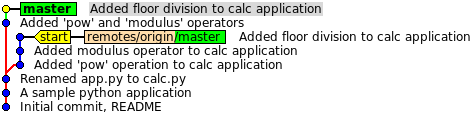
\includegraphics[width=0.75\linewidth]{gitrebase-squash.png}
  \label{fig:gitrebase-squash}
  \caption{Resultat d'un squash lors de git rebase}
\end{figure*}

Réinitialisons notre branche une nouvelle fois avant la prochaine partie:

\begin{lstlisting}[style=BashInputStyle]
  git reset --hard origin/master
\end{lstlisting}

\noindent \textbf{Découper un commit}
Il est possible de découper un commit en plusieurs commits, mais c'est un peu plus compliqué.
Le mot-clé à utiliser dans l'éditeur interactif est \textbf{edit}, comme nous l'avons déjà effectué pour modifier le message de commit.
Supposont que nous voulions séparer le commit implémentant l'opération de modulo, nous pouvons rebase jusqu'à HEAD\textasciitilde2:

\begin{lstlisting}[style=BashInputStyle]
  $ git rebase -i HEAD~2
\end{lstlisting}

Dans l'éditeur de rebase, notons \textbf{edit} sur 511d31d

\begin{lstlisting}[style=BashInputStyle]
  edit 511d31d Added modulus operator to calc application
  pick 87854e9 New message
\end{lstlisting}

Git s'arrêtera après l'application du commit 511d31d.
\textbf{La partie subtile:} Git a déjà appliqué le commit en entier, et la pause est marquée pour rajouter d'autres modifications à l'index ou pour éditer le message. Comment donc découper le commit en plusieurs?
\marginnote{oui, un reset durant un rebase est tout à fait possible}
Le développeur doit maintenant \textbf{reset} sur HEAD\textasciitilde1, ce qui aura pour effet de défaire le commit venant d'être appliqué. Les modifications seront en l'état \texttt{modified} car nous avons utilisé la commande reset normale, sans l'option \texttt{soft}.

\begin{lstlisting}[style=BashInputStyle]
  $ git reset HEAD~1
\end{lstlisting}

\marginnote{rappelez-vous à quel point git add -p est utile pour indexer du code partiellement}
Vous pouvez à présent \textbf{git add} les modifications partiellement, puis commit, indexer davantage, commit, etc jusqu'à ce que tout a été indexé et committé:

\begin{lstlisting}[style=BashInputStyle]
  $ git add -p
  # stage part of the modifications
  $ git commit -m "modulus implementation, phase 1"
  $ git add -p
  # stage part of the modifications
  $ git commit -m "modulus implementation, phase 2"
  $ git rebase --continue
\end{lstlisting}

La branche \texttt{master} locale contiendra plusieurs commits résultants de la séparation:

\begin{figure*}%
  \centering
  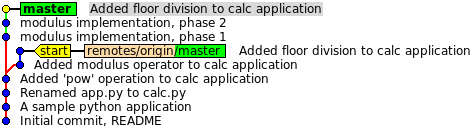
\includegraphics[width=0.75\linewidth]{gitrebase-split.png}
  \label{fig:gitrebase-split}
  \caption{Résultat d'un découpage de commit lors d'un rebase}
\end{figure*}

\noindent \textbf{Supprimer et permuter des commit}

Enfin, il est possible de supprimer et réordonner des commits.
Pour cela, il suffit de supprimer et de permuter des lignes de l'éditeur de commit interactif. \marginnote{attention: contrairement aux autres opérations vues jusqu'à présent, cela ne sera pas toujours possible car il pourrait y avoir des conflits.}
Ceci est laissé à titre d'exercice.

\bibliography{../common/refs}
\bibliographystyle{plainnat}

\end{document}